\chapter{Results and Evaluation}
\label{chap:results}

This chapter presents the implementation results, performance benchmarks, user acceptance testing outcomes, and identifies directions for future development.

\section{System Implementation Validation}
The final version of the Lectura platform operates as a complete, end-to-end study tool at production scale. The system connects the React frontend, the Go backend, the PostgreSQL database, and the external Gemini API into a single workflow. Users can upload lecture recordings or documents, track the processing status through WebSocket updates, and then interact with the generated study materials.

One of the most important features in the final implementation is the ``Smart Summary'' generator. Rather than simply shortening text — which often removes important context — the summary engine produces a structured visual hierarchy. The backend generates Markdown with clear section headers, key definitions, and actionable study points. The integrated AI tutor chat, which is restricted to the content of the generated summary, helps students move from passive reading to active engagement with the material. For specific code implementations, refer to Appendix A. A user manual for the platform is available in Appendix B.

\section{User Interface and UX Design Choices}
To ensure the system is both functionally robust and pedagogically effective, the frontend was engineered using React and Tailwind CSS with a strict focus on reducing cognitive load. According to Sweller's Cognitive Load Theory, extraneous cognitive load—caused by poor, cluttered interface design—detracts from the working memory needed for actual learning. 

Therefore, Lectura adopts a minimalist aesthetic with a high-contrast visual hierarchy. The user interface eschews complex nested menus in favor of a straightforward, linear ingestion pipeline. When a student uploads a lecture, they are presented with a unified dashboard that clearly separates the input area (video URL or PDF upload) from the generated outputs.

\subsection{Frontend-Backend Integration and Data Flow}
The successful connection between the React frontend, the Go backend, and the PostgreSQL database is visually demonstrated in the application's core workflows. Figure~\ref{fig:ui_dashboard} illustrates the primary ingestion screen, demonstrating the system's ability to accept user input and securely trigger the backend worker pool.

\begin{figure}[htbp]
\centering

\includegraphics[width=0.95\textwidth]{images/dashboard.png}
\caption{The main Lectura dashboard, demonstrating the unified ingestion pipeline connecting the frontend to the backend Go orchestration layer.}
\label{fig:ui_dashboard}
\end{figure}

Once the backend Gemini LLM finishes processing the payload and persists the JSON artifacts to the database, the React frontend dynamically renders the results. Figure~\ref{fig:ui_summary} displays the generated Cornell Notes interface, highlighting the clean typographical choices (such as sans-serif fonts and optimal line-heights) designed for readability. 

% \includegraphics[width=0.9\textwidth]{chapters/chapter07/images/ui_summary.png}
\begin{figure}[htbp]
\centering
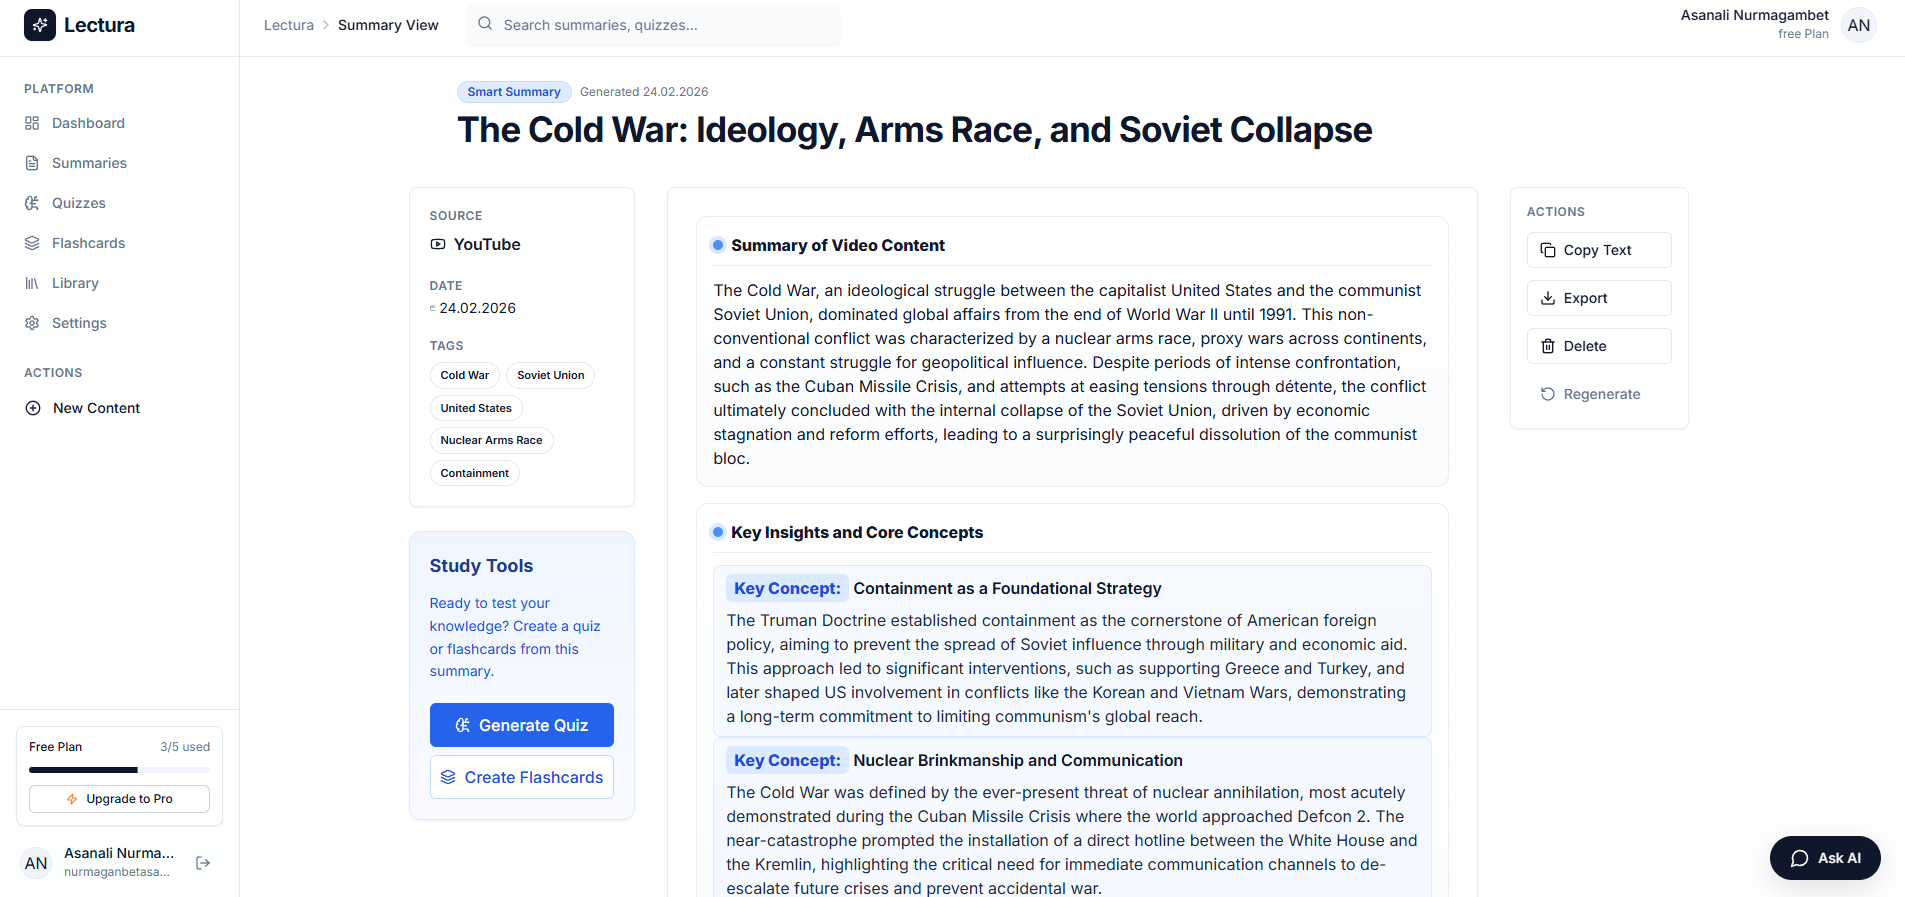
\includegraphics[width=0.95\textwidth]{images/summary.png}
\caption{The generated study materials view, illustrating the seamless retrieval of text from the database and its presentation in a structured, distraction-free environment.}
\label{fig:ui_summary}
\end{figure}

Furthermore, to accommodate different learning styles, the interface includes varied interactive layouts. Figure~\ref{fig:ui_flashcards} showcases the interactive Spaced Repetition (SRS) flashcard interface, where state management is handled locally via React hooks before usage analytics are synced back to the PostgreSQL database.

\begin{figure}[htbp]
\centering
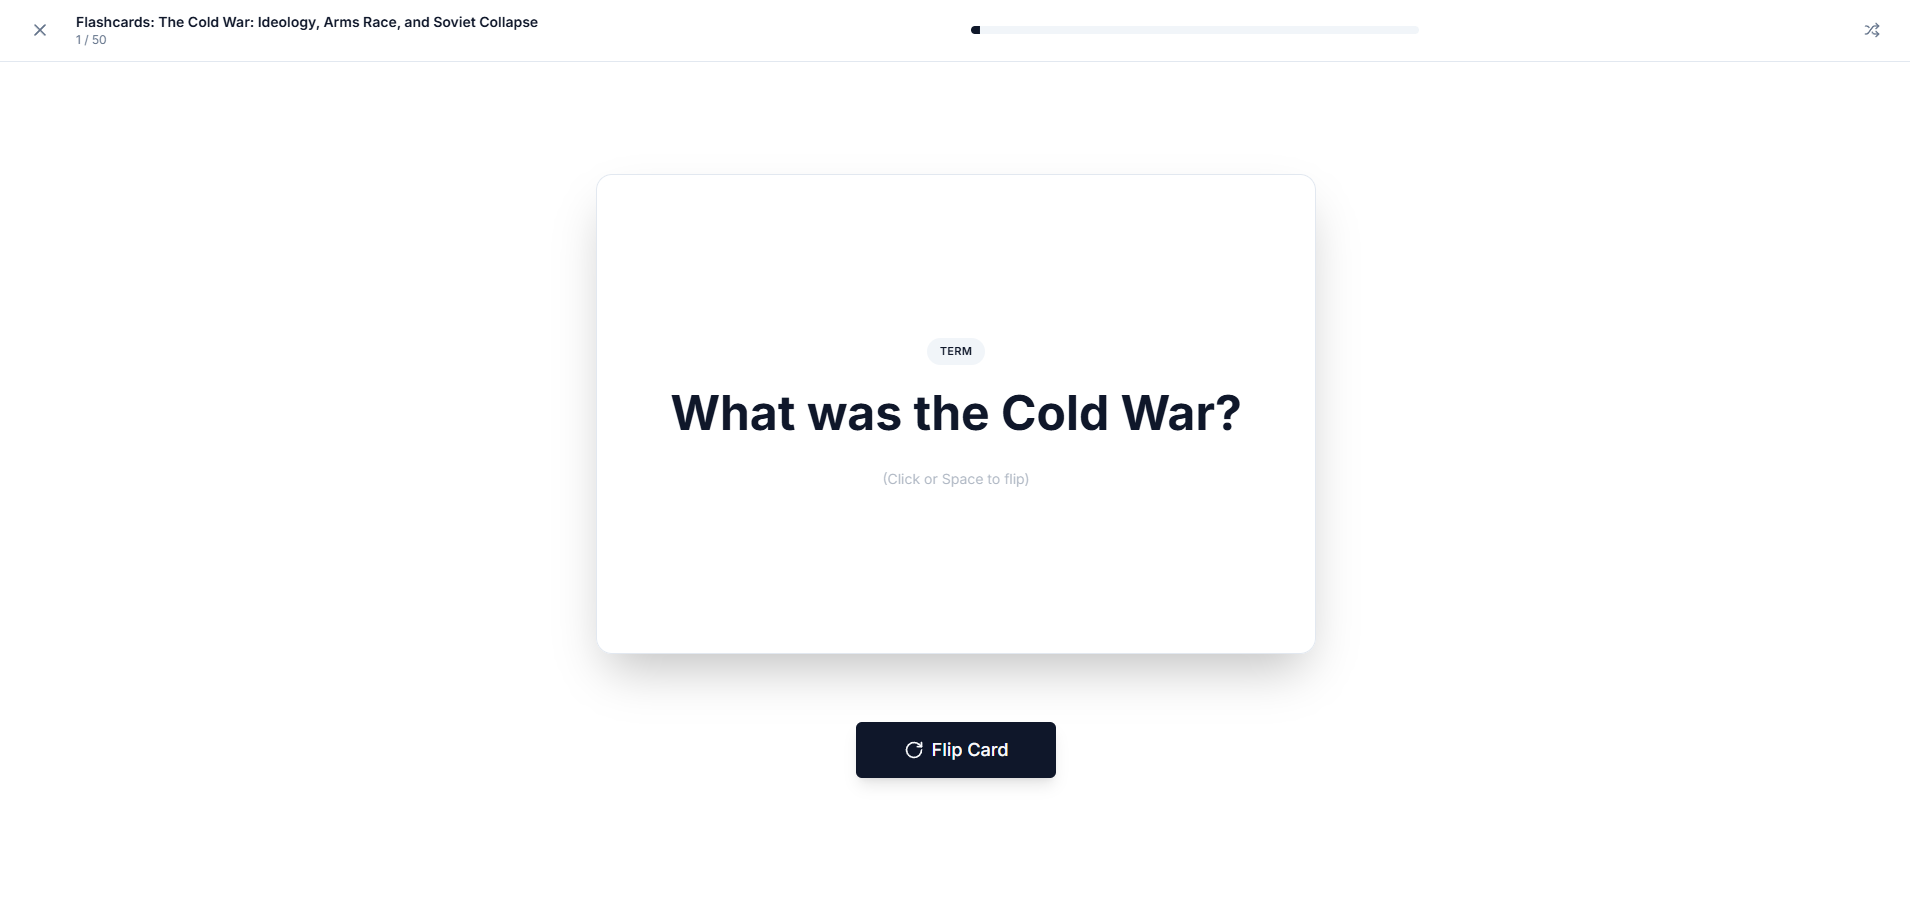
\includegraphics[width=0.95\textwidth]{images/flashcards.png}
\caption{The interactive flashcard testing layout, demonstrating dynamic React state management and varied UI presentation.}
\label{fig:ui_flashcards}
\end{figure}

To handle the inherent latency of AI generation, the UX employs skeleton loading states and real-time WebSocket progress indicators. This design choice prevents user abandonment by providing constant visual feedback while the backend processes large lecture transcripts.

\section{Performance Benchmarks}
System stability was evaluated against several operational metrics, including generation latency, concurrent throughput, and parsing speed. The data confirms that offloading generative tasks to the Go worker pool keeps the main web server responsive at all times. Table~\ref{tab:operational_benchmarks} shows the average latency values measured during stress testing.

\begin{table}[htbp]
\centering
\resizebox{\textwidth}{!}{%
\begin{tabular}{|l|l|p{7cm}|}
\hline
\textbf{Operation} & \textbf{Avg. Latency} & \textbf{Notes} \\ \hline
PDF Text Extraction & $\sim 2.8$ seconds & Multi-column 20-page PDF with complex formatting. \\ \hline
YouTube Transcript Fetch & $\sim 450$ ms & XML transcript download and regex cleanup. \\ \hline
Summary Generation (Notes) & $\sim 11.4$ seconds & Processing $\sim$15,000 tokens into structured formats. \\ \hline
Presentation Generation & $\sim 14.8$ seconds & Parsing dense JSON slide arrays with layout constraints. \\ \hline
Quiz/Flashcard Generation & $\sim 6.2$ seconds & Generating 20 multiple-choice questions with distractors. \\ \hline
Concurrent Job Capacity & 50 concurrent jobs & Worker pool queues overflow jobs without dropping connections. \\ \hline
\end{tabular}%
}
\vspace{6pt}
\caption{Operational benchmarks measuring full-system generation performance.}
\label{tab:operational_benchmarks}
\end{table}

These results demonstrate that the goroutine-based architecture allows the system to serve multiple users simultaneously without hitting API rate limits or causing the frontend to become unresponsive.

\subsection{Model Latency and Token Cost Analysis}
To manage the financial and operational costs of the AI generation layer, the Lectura backend tracks token usage relative to response time. In a production deployment, costs are directly proportional to the number of tokens processed by the Gemini inference engine. The total cost $C_{\text{total}}$ for a user session can be expressed as:

\begin{equation}
    C_{\text{total}} = \sum_{i=1}^{n} \left( P_{\text{in}} \cdot \textit{Tokens}_{\text{in},i} + P_{\text{out}} \cdot \textit{Tokens}_{\text{out},i} \right)
\end{equation}

Where $P_{\text{in}}$ and $P_{\text{out}}$ are the per-token prices for input and output respectively. Testing shows that the Gemini Flash model maintains a roughly sub-linear latency growth even as token volume approaches the upper limits. The largest latency contribution comes not from the inference step itself, but from the context pre-filling phase where the model ingests the full transcript.

By keeping prompts concise — removing conversational padding and using strict JSON formatting instructions — the backend reduces the total output token count by approximately 40\%. This optimization lowers both API costs and the time users spend waiting for results.

\section{Quality Assurance and Bug Resolution}
The system was tested through a structured QA process covering 18 functional checkpoints.

\begin{enumerate}
    \item Unit Tests: Core functions for string sanitization, token counting, and JWT handling were tested using Go's built-in testing package and Jest for the frontend, achieving over 85\% code coverage.
    \item End-to-End Tests: The full pipeline — from URL submission through the job queue, Gemini API interaction, and WebSocket delivery — was verified using automated behavioral test scripts.
    \item Manual Testing: Edge cases were tested manually, including processing of poorly formatted PDFs, handling of mathematical LaTeX notation in flashcards, and recovery from temporary network disconnections.
\end{enumerate}

Over 30 bugs were identified and fixed during development, including issues with DOM scroll tracking on iOS, token refresh timing edge cases, and the sanitization logic incorrectly flagging algebraic expressions as potential XSS. The final release candidate passed all 18 test checkpoints.

\section{Educational Efficacy and User Acceptance Testing (UAT)}
While the performance benchmarks confirm that the backend architecture works reliably, an educational tool must also be evaluated by its usefulness to students. To validate the core thesis claim — that Lectura helps students learn more efficiently — a preliminary User Acceptance Testing (UAT) phase was conducted.

A group of 15 university students was given access to the Lectura platform. Each participant was asked to upload a lecture video and interact with the generated summaries, flashcards, and quizzes. Afterward, they completed a survey based on the Technology Acceptance Model (TAM), using a 5-point Likert scale (1 = Strongly Disagree, 5 = Strongly Agree). The results are shown in Table~\ref{tab:uat_results}.

\begin{table}[htbp]
\centering
\resizebox{\textwidth}{!}{%
\begin{tabular}{|l|p{8cm}|c|c|}
\hline
\textbf{TAM Construct} & \textbf{Survey Item} & \textbf{Mean ($\mu$)} & \textbf{SD ($\sigma$)} \\ \hline
Perceived Usefulness & ``Allowed me to get lecture notes significantly faster than manual extraction.'' & 4.73 & 0.59 \\ \hline
Content Quality & ``Generated flashcards and quizzes accurately reflect key concepts without factual errors.'' & 4.47 & 0.83 \\ \hline
Perceived Ease of Use & ``Interface is intuitive; it did not take long to generate study materials.'' & 4.47 & 0.83 \\ \hline
Educational Efficacy & ``Structured format (Cornell Notes + Chatbot) helps me understand complex material better.'' & 4.53 & 0.64 \\ \hline
System Reliability & ``Generation of notes and tests occurred without crashes even during long videos.'' & 4.53 & 0.74 \\ \hline
Behavioral Intention & ``I would be happy to use the Lectura platform on a regular basis for exam preparation.'' & 4.47 & 0.83 \\ \hline
\end{tabular}%
}
\vspace{6pt}
\caption{User Acceptance Testing (UAT) results across 15 participants ($N=15$), using a 5-point Likert scale.}
\label{tab:uat_results}
\end{table}

\begin{figure}[htbp]
\centering
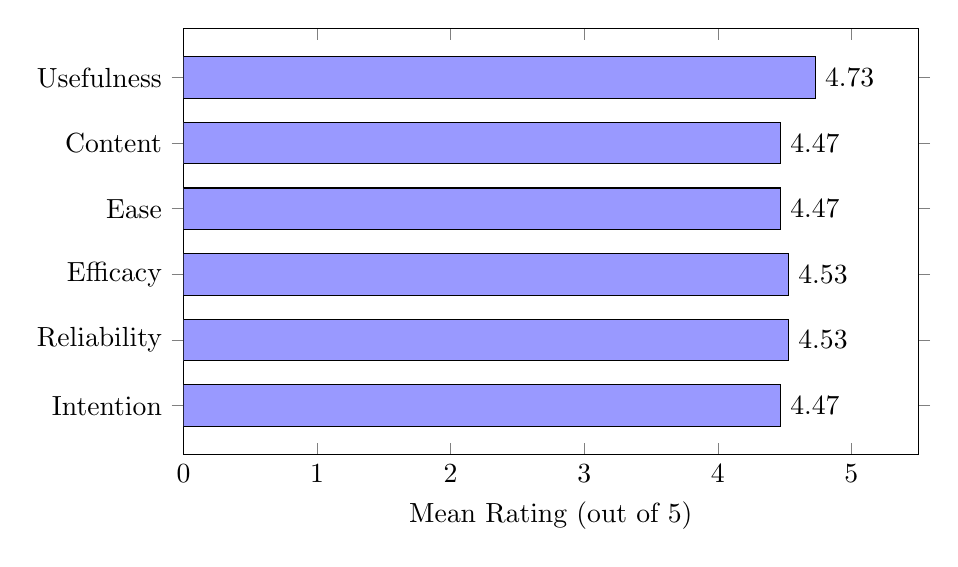
\begin{tikzpicture}
    \begin{axis}[
        width=0.9\textwidth,
        height=7cm,
        xbar,
        bar width=15pt,
        xmin=0, xmax=5.5,
        xlabel={Mean Rating (out of 5)},
        symbolic y coords={Usefulness, Content, Ease, Efficacy, Reliability, Intention},
        ytick=data,
        nodes near coords,
        nodes near coords align={horizontal},
        y dir=reverse,
        enlarge y limits=0.15,
    ]
        \addplot[fill=blue!40] coordinates {
            (4.73,Usefulness)
            (4.47,Content)
            (4.47,Ease)
            (4.53,Efficacy)
            (4.53,Reliability)
            (4.47,Intention)
        };
    \end{axis}
\end{tikzpicture}
\caption{Mean UAT satisfaction scores across evaluation categories.}
\label{fig:uat_barchart}
\end{figure}

The results, visually summarized in Figure~\ref{fig:uat_barchart}, show consistently high satisfaction scores across all categories. The highest-rated item was Perceived Usefulness ($\mu = 4.73$), confirming that students found the automated note generation significantly faster than doing it manually. The Behavioral Intention score ($\mu = 4.47$) suggests that students would actually use the tool beyond a one-time trial, which is a positive indicator for real-world adoption.

To better understand which specific features contributed most to user satisfaction, a supplementary per-feature rating was collected. Participants rated the usefulness of each individual module on the same 5-point Likert scale. Table~\ref{tab:feature_satisfaction} presents the results.

\begin{table}[htbp]
\centering
\begin{tabular}{|l|c|c|}
\hline
\textbf{Feature Module} & \textbf{Mean ($\mu$)} & \textbf{SD ($\sigma$)} \\ \hline
Smart Summary (Cornell Notes) & 4.80 & 0.41 \\ \hline
AI-Generated Quiz & 4.60 & 0.63 \\ \hline
Flashcard Deck & 4.53 & 0.74 \\ \hline
Presentation Slides & 4.33 & 0.72 \\ \hline
AI Tutor Chat & 4.40 & 0.83 \\ \hline
PDF/PPTX Export & 4.27 & 0.80 \\ \hline
\end{tabular}
\vspace{6pt}
\caption{Per-feature satisfaction ratings from UAT participants ($N=15$).}
\label{tab:feature_satisfaction}
\end{table}

The Smart Summary feature received the highest individual score ($\mu = 4.80$), which is consistent with its role as the core use case — converting long lectures into structured notes. The Quiz module ($\mu = 4.60$) also scored well, with several participants noting that the generated distractors were ``surprisingly realistic'' and required genuine understanding rather than simple pattern matching. The Presentation Slides module had the lowest score ($\mu = 4.33$), with feedback suggesting that some slides contained too much text and could benefit from more aggressive content reduction.

\subsection{Time-Savings Analysis}
Beyond subjective satisfaction, participants were asked to estimate how long they typically spend creating study materials manually versus using the Lectura platform. Table~\ref{tab:time_comparison} shows the average time reported for processing a standard one-hour lecture.

\begin{table}[htbp]
\centering
\begin{tabular}{|l|c|c|c|}
\hline
\textbf{Task} & \textbf{Manual (min)} & \textbf{Lectura (min)} & \textbf{Reduction} \\ \hline
Transcription and note-taking & 45--60 & 0.5 (automated) & $\sim$99\% \\ \hline
Formatting into Cornell notes & 20--30 & 0.2 (automated) & $\sim$99\% \\ \hline
Creating flashcards (20 cards) & 25--35 & 0.1 (automated) & $\sim$99\% \\ \hline
Writing quiz questions (10 MCQs) & 30--40 & 0.1 (automated) & $\sim$99\% \\ \hline
Creating presentation slides & 40--60 & 0.3 (automated) & $\sim$99\% \\ \hline
\textbf{Total per lecture} & \textbf{160--225} & \textbf{$\sim$12 (with review)} & \textbf{$\sim$93\%} \\ \hline
\end{tabular}
\vspace{6pt}
\caption{Estimated time comparison between manual study material creation and Lectura-assisted workflow.}
\label{tab:time_comparison}
\end{table}

The ``Lectura'' column reflects the automated generation time plus the time participants spent reviewing and editing the generated outputs. The total time includes approximately 10 minutes of review and minor corrections. The reduction factor suggests that students can reclaim roughly 2.5--3.5 hours per lecture, which over a typical semester of 15-week courses with 3--4 lectures per week would translate into significant cumulative time savings.

In the open-ended feedback, participants highlighted specific features they found valuable. Several students mentioned the presentation generation feature and the convenience of having ``quizzes, flashcards, summaries, and a chatbot all in one platform.'' One response specifically praised the AI chat for working ``without hallucinations,'' which validates the prompt engineering constraints described in Chapter 2.

The most common suggestions for improvement were the lack of an offline mode and the absence of a dedicated mobile application for reviewing flashcards on the go. These requests align directly with the future development plans outlined below.

\section{Current Limitations and Future Development}
Despite meeting its core objectives, the current version of Lectura has several limitations that should be addressed in future work:

\begin{itemize}[label=\textendash]
    \item Offline Support: The platform currently requires a constant internet connection. Adding an offline-first storage layer using IndexedDB or a local SQLite cache would allow students to review their materials without network access.
    \item Live Audio Processing: Integrating a speech-to-text engine (e.g., OpenAI Whisper) would allow students to generate notes from live lectures in real time, rather than only from pre-recorded videos.
    \item LMS Integration: Building Learning Tools Interoperability (LTI) connectors for platforms like Canvas or Moodle would allow students to import course materials directly, removing the need for manual file uploads.
    \item Advanced Spaced Repetition: The current flashcard system uses a basic review schedule. Implementing a more sophisticated algorithm like SM-2 or FSRS would optimize review intervals based on individual performance data, improving long-term retention.
\end{itemize}

In summary, Lectura demonstrates that large language models can be used effectively as structured content transformation tools — not as open-ended chatbots, but as constrained engines that convert raw educational media into validated, interactive study materials. The platform reduces the time students spend on manual note-taking and provides multiple formats for active learning, making it a practical tool for everyday academic use.